%! Author = gramic
%! Date = 15.03.24

% Preamble
\begin{flushleft}
    \subsubsection{yugabyteDB}
    \paragraph{Installation}
    Wähend der Installation des YugabyteDB Evaluations-Enviroment wurde festgestellt, das man zwei Varianten Installieren kann.
    YugabyteDB (Repository yugabyte) und YugabyteDB Anywhere (Repository yugawre)

    \begin{figure}[H]
        \centering
        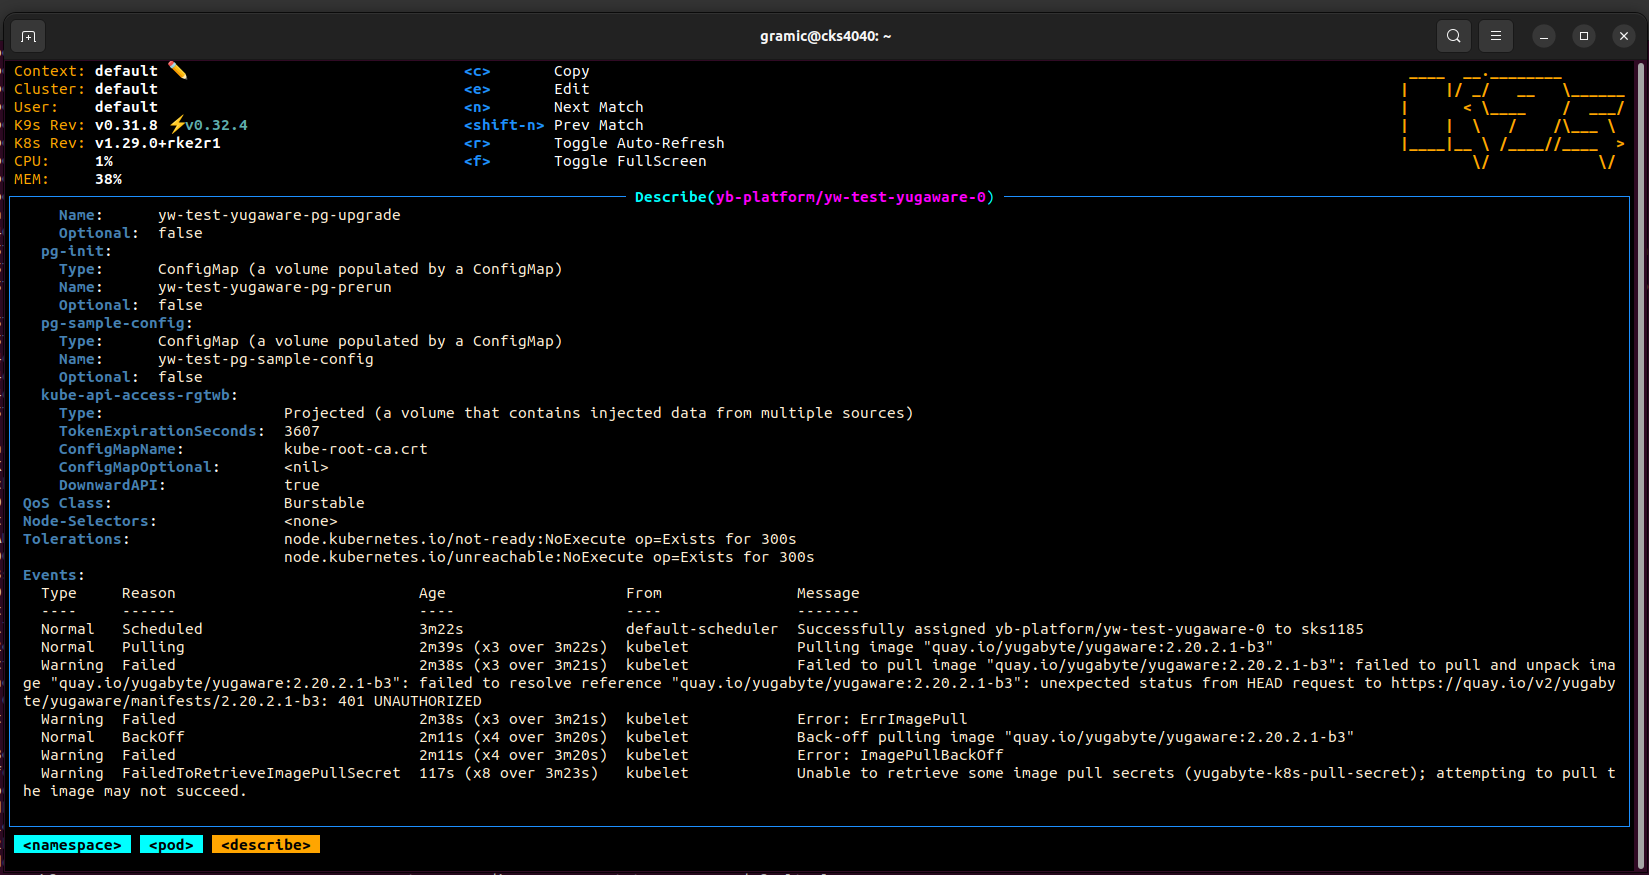
\includegraphics[width=1\linewidth]{source/implementation/evaluation/platforms/yugabytedb_pod_installation_subscription_interrup}
        \caption{yugabyteDB - Susbsription yugawre}
        \label{fig:yugabytedb_pod_installation_subscription_interrup}
    \end{figure}

    Es stellte sich auch heraus, dass wenn man YugabyteDB 4 Cores pro Node zur Verfügung geben will (je zwei für den \texttt{master} und \texttt{tserver}),\\
    der Server mehr als 4 Cores haben muss.\\
    Andernfalls wird Kubernetes einen der beiden Pods nicht deployen, weil zuwenig Cores zur verfügung stehen.
\end{flushleft}

\begin{flushleft}
    \paragraph{Konfiguration}
    Damit nicht der YugabyteDB Anywhere-Service installiert wird, muss das entsprechende Image gesetzt werden:
    \lstset{style=gra_codestyle}
    \begin{lstlisting}[language=yaml, caption=yugabyteDB - Helm Chart Manifest - Detail Image,captionpos=b,label={lst:yugabytedb-image-setting},breaklines=true]
...
Image:
  repository: "yugabytedb/yugabyte"
  tag: 2.20.2.1-b3
  pullPolicy: IfNotPresent
  pullSecretName: ""
...
    \end{lstlisting}

    Die StorageClass muss im \texttt{values.yaml} gesetzt werden, einmal für den \texttt{master} und einmal für den \texttt{tserver}
    \lstset{style=gra_codestyle}
    \begin{lstlisting}[language=yaml, caption=yugabyteDB - Helm Chart Manifest - Detail StorageClass,captionpos=b,label={lst:yugabytedb-storageclass-setting},breaklines=true]
...
storage:
  ephemeral: false  # will not allocate PVs when true
  master:
    count: 1
    size: 3Gi
    storageClass: "yb-storage"
  tserver:
    count: 1
    size: 3Gi
    storageClass: "yb-storage"
...
    \end{lstlisting}

    Dem node werden je 4 Cores zur verfügung gestellt.
    Zei für den \texttt{master} und zwei für den \texttt{tserver}.
    Beide erhalten 4GiB Memory:
    \lstset{style=gra_codestyle}
    \begin{lstlisting}[language=yaml, caption=yugabyteDB - Helm Chart Manifest - Detail Resources,captionpos=b,label={lst:yugabytedb-resources-setting},breaklines=true]
...
resource:
  master:
    requests:
      cpu: "1"
      memory: 2Gi
    limits:
      cpu: "1"
      ## Ensure the 'memory' value is strictly in 'Gi' or 'G' format. Deviating from these formats
      ## may result in setting an incorrect value for the 'memory_limit_hard_bytes' flag.
      ## Avoid using floating numbers for the numeric part of 'memory'. Doing so may lead to
      ## the 'memory_limit_hard_bytes' being set to 0, as the function expects integer values.
      memory: 2Gi
  tserver:
    requests:
      cpu: "1"
      memory: 4Gi
    limits:
      cpu: "1"
      ## Ensure the 'memory' value is strictly in 'Gi' or 'G' format. Deviating from these formats
      ## may result in setting an incorrect value for the 'memory_limit_hard_bytes' flag.
      ## Avoid using floating numbers for the numeric part of 'memory'. Doing so may lead to
      ## the 'memory_limit_hard_bytes' being set to 0, as the function expects integer values.
      memory: 4Gi
...
    \end{lstlisting}

    Die Shards, oder Tablets wie sie Yugabyte nennt, sollen auf allen drei Nodes repliziert werden:
    \lstset{style=gra_codestyle}
    \begin{lstlisting}[language=yaml, caption=yugabyteDB - Helm Chart Manifest - Detail Replika,captionpos=b,label={lst:yugabytedb-replica-setting},breaklines=true]
...
replicas:
  master: 3
  tserver: 3
  ## Used to set replication factor when isMultiAz is set to true
  totalMasters: 3
...
    \end{lstlisting}

    Wichtig ist auch, dass der \texttt{YSQL}-Dienst aktiv ist, damit PostgreSQL Abfragen abgesetzt werden können.\\
    Deshalb muss der Dienst aktiv sein und darf nicht deaktiviert werden:
    \lstset{style=gra_codestyle}
    \begin{lstlisting}[language=yaml, caption=yugabyteDB - Helm Chart Manifest - Detail Disable YSQL,captionpos=b,label={lst:yugabytedb-disableYsql-setting},breaklines=true]
...
# Disable the YSQL
disableYsql: false
...
    \end{lstlisting}

    Nun muss die Domain und die Service-Endpoints konfiguriert werden.\\
    Der Domainname bleibt vorerst \texttt{cluster.local} wie Default hinterlegt.\\
    Die Servicenamen und Ports werden nicht angetastet, wichtig ist die LoadBalancer-IP.\\
    Sie ist entsprechend der gewählten VirtualIP mit \texttt{10.0.20.106} zu setzen.

    \lstset{style=gra_codestyle}
    \begin{lstlisting}[language=yaml, caption=yugabyteDB - Helm Chart Manifest - Detail Domainname und Service-Endpoints,captionpos=b,label={lst:yugabytedb-domainname-serviceendpoints-setting},breaklines=true]
...
domainName: "cluster.local"

serviceEndpoints:
  - name: "yb-master-ui"
    type: LoadBalancer
    annotations: {}
    clusterIP: ""
    ## Sets the Service's externalTrafficPolicy
    externalTrafficPolicy: ""
    app: "yb-master"
    loadBalancerIP: ""
    ports:
      http-ui: "7000"

  - name: "yb-tserver-service"
    type: LoadBalancer
    annotations:
      metallb.universe.tf/loadBalancerIPs: 10.0.20.106
    clusterIP: ""
    ## Sets the Service's externalTrafficPolicy
    externalTrafficPolicy: ""
    app: "yb-tserver"
    loadBalancerIP: ""
    ports:
      tcp-yql-port: "9042"
      tcp-yedis-port: "6379"
      tcp-ysql-port: "5433"
...
    \end{lstlisting}

\end{flushleft}
\begin{flushleft}


    \paragraph{Connection}
    Der Connect via JDBC ist nicht ohne weiteres möglich.
    Bei DataGrip muss der spezielle Driver ausgewählt werden.
\end{flushleft}